\chapter{Dataset}
\label{chap:dataset}
In this chapter, we present the dataset used in our work.
We use the \gls{scid} dataset \cite{ni_esim_2017}\footnote{The dataset can be downloaded here: https://eezkni.github.io/publications/ESIM.html.} as the base for our experiments.
The \gls{scid} dataset is suitable for our work, since the images contain text content on screenshots, different distortion levels and \gls{mos} values for each image.
Among the available screen content datasets mentioned in the literature \cite{iqa_survey_2020}, we find that other options are either inaccessible or fail to fulfill all the necessary criteria we require for our research.
An overview of the 40 reference images of the dataset can be seen in \autoref{fig:dataset_overview}.
Additionally, the dataset contains 1800 distorted images, which we discuss in the next section in detail.
The dataset includes a \gls{mos} for each of the distorted images, which represents the perceived quality by a human observer.
The subjective tests were conducted using the double stimulus method, involving the following steps.
First, the reference image was shown to the candidates for 10 seconds, followed by a mid-gray screen.
Afterwards, the distorted image was shown for 10 seconds.
Finally, the candidates were asked to rate the distorted image's quality compared to the reference image on a 5-point scale, 1 being the worst and 5 being the best.
These scores are then converted to a \gls{mos} value for each image between 0 and 100, with 100 representing the highest quality.



\begin{figure}[h!]
    \centering
    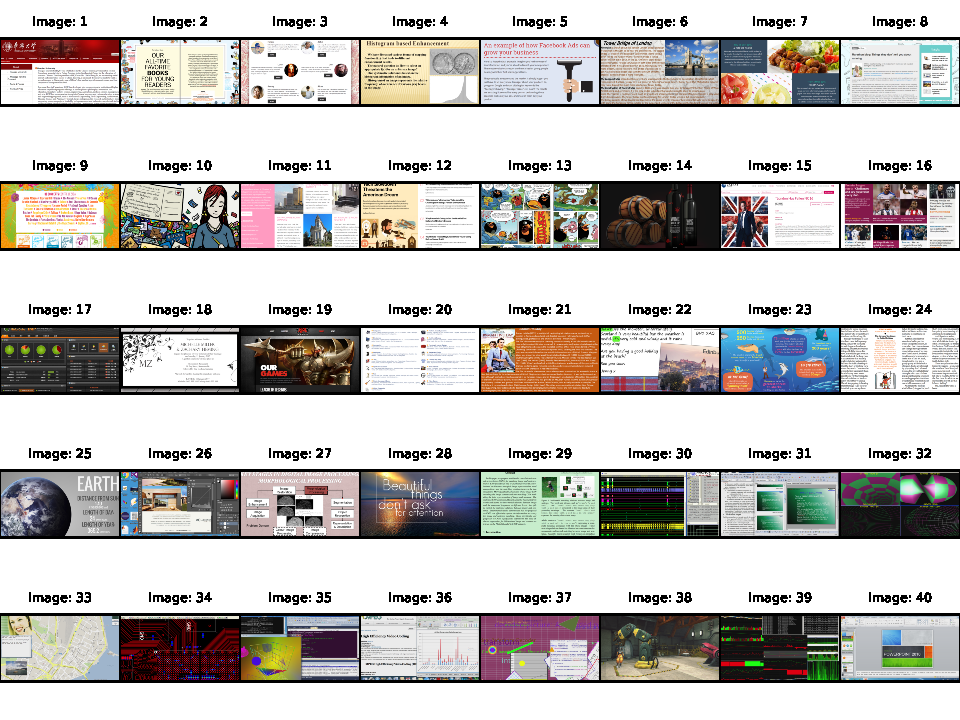
\includegraphics[width=\textwidth]{reference_images}
    \caption{Overview of the dataset.}
    \label{fig:dataset_overview}
\end{figure}


\section{Distortion types}
\label{sec:dataset_distortion_types}


The 1800 distorted images are generated from the 40 reference images.
They are distorted with 9 different distortion types, each with 5 different distortion quality levels.
In \autoref{tab:distortion_types}, we list the distortion types with a short description.


\begin{table}[h!]
\centering
\caption{Overview of the distortion types used in the dataset.}
\begin{tabular}{|p{6cm}|c|p{6cm}|}
\hline
\textbf{Distortion Type} & \textbf{Abbreviation} & \textbf{Description} \\
\hline
\hline
Gaussian Noise & GN & Addition of noise to an image using a Gaussian distribution \\
\hline
Gaussian Blur & GB & Blurring of an image using a Gaussian kernel \\
\hline
Motion Blur & MB & Blurring of an image due to movement of the camera or the object \\
\hline
Contrast Change & CC & Change in the contrast of an image \\
\hline
Joint Photographic Experts Group & JPEG & Image compression standard \\
\hline
Joint Photographic Experts Group 2000 & JPEG2000 & Image compression standard \\
\hline
Color Saturation Change & CSC & Changes in the color saturation of an image \\
\hline
High Efficiency Video Coding-Screen Content Coding & HEVC-SCC & Video compression standard for screen content \\
\hline
Color Quantization with Dithering & CQD & Reduction of colors available in an image \\
\hline
\end{tabular}
\label{tab:distortion_types}
\end{table}


The images distorted by \gls{gn} have noise added with zero mean and standard deviations of $0.001$, $0.005$, $0.01$, $0.05$ and $0.1$ for each quality level respectively.
The images distorted by \gls{gb} are blurred with a Gaussian kernel.
The size of the kernel is $5\times5$ with standard deviations of $0.58$, $0.76$, $0.96$, $1.2$ and $2.1$ for each quality level respectively.
Images distorted by \gls{mb} are blurred with a motion kernel, which simulates motion blur.
The 'theta' parameter, which controls the degree of angle in a counter-clockwise direction, is set to zero and the 'len' parameter, which determines the length of the movement of the simulated camera, is set to $2$, $3.4$, $4$, $5.5$ and $6.4$ respectively.
The \gls{cc} distortion scales certain pixel values in the reference image to new values to change the contrast.
The scaling is applied for the ranges $[0,1] \rightarrow [0.3,0.5]$, $[0,1] \rightarrow [0.1,0.7]$, $[0.1,0.8] \rightarrow [0.1,0.9]$, $[0.2,0.8] \rightarrow [0.1,0.8]$ and $[0.2,0.7] \rightarrow [0,1]$ respectively.
So for the first quality level, all pixel values (from 0 to 1) are scaled to values between 0.3 and 0.5 of the maximum pixel intensity.
For the \gls{jpeg} compression, the images are compressed by the image compression algorithm with quality factors $75$, $35$, $18$, $8$ and $5$ respectively.
The \gls{jpeg2000} compression is applied with compression ratios of $0.08$, $0.045$, $0.02$, $0.015$ and $0.01$ respectively.
The \gls{csc} distortion keeps the luminance component of the images constant, but scales the chrominance components by the factors $0.96$, $0.72$, $0.58$, $0.42$ and $0.1$ respectively.
The \gls{hevcscc} distortion is applied by using the \gls{hevc} codec with the screen content configuration on the images with \glspl{qp} set to $16$, $36$, $40$, $42$ and $48$ respectively.
The \gls{cqd} distortion is applied by reducing the number of colors available in the image to $30$, $28$, $25$, $10$ and $5$ respectively.
More detailed descriptions of the implementation of the distortions can be found in the supporting file included with the dataset.
The different distortion types, at their most severe quality level, can be seen in \autoref{fig:distortion_types}, applied to the image in \autoref{fig:img29}.

\begin{figure}[h!]
    \centering
    \includegraphics[width=\textwidth]{../../data/raw/scid/ReferenceSCIs/SCI29.png}
    \caption{Reference image SCI29}
    \label{fig:img29}
\end{figure}

\begin{figure}[h!]
    \centering
    \begin{subfigure}[b]{0.3\textwidth}
        \includegraphics[width=\textwidth]{../../data/raw/scid/DistortedSCIs/SCI29_1_5.png}
        \caption{Gaussian Noise}
        \label{fig:distortion_type_1}
    \end{subfigure}
    \hfill
    \begin{subfigure}[b]{0.3\textwidth}
        \includegraphics[width=\textwidth]{../../data/raw/scid/DistortedSCIs/SCI29_2_5.png}
        \caption{Gaussian Blur}
        \label{fig:distortion_type_2}
    \end{subfigure}
    \hfill
    \begin{subfigure}[b]{0.3\textwidth}
        \includegraphics[width=\textwidth]{../../data/raw/scid/DistortedSCIs/SCI29_3_5.png}
        \caption{Motion Blur}
        \label{fig:distortion_type_3}
    \end{subfigure}
    \newline
    \begin{subfigure}[b]{0.3\textwidth}
        \includegraphics[width=\textwidth]{../../data/raw/scid/DistortedSCIs/SCI29_4_5.png}
        \caption{Contrast Change}
        \label{fig:distortion_type_4}
    \end{subfigure}
    \hfill
    \begin{subfigure}[b]{0.3\textwidth}
        \includegraphics[width=\textwidth]{../../data/raw/scid/DistortedSCIs/SCI29_5_5.png}
        \caption{JPEG Compression}
        \label{fig:distortion_type_5}
    \end{subfigure}
    \hfill
    \begin{subfigure}[b]{0.3\textwidth}
        \includegraphics[width=\textwidth]{../../data/raw/scid/DistortedSCIs/SCI29_6_5.png}
        \caption{JPEG2000 Compression}
        \label{fig:distortion_type_6}
    \end{subfigure}
    \newline
    \begin{subfigure}[b]{0.3\textwidth}
        \includegraphics[width=\textwidth]{../../data/raw/scid/DistortedSCIs/SCI29_7_5.png}
        \caption{Color Saturation Change}
        \label{fig:distortion_type_7}
    \end{subfigure}
    \hfill
    \begin{subfigure}[b]{0.3\textwidth}
        \includegraphics[width=\textwidth]{../../data/raw/scid/DistortedSCIs/SCI29_8_5.png}
        \caption{HEVC Screen Content Coding}
        \label{fig:distortion_type_8}
    \end{subfigure}
    \hfill
    \begin{subfigure}[b]{0.3\textwidth}
        \includegraphics[width=\textwidth]{../../data/raw/scid/DistortedSCIs/SCI29_9_5.png}
        \caption{Color Quantization with dithering}
        \label{fig:distortion_type_9}
    \end{subfigure}
    \caption{Distorted image 29 with 9 different distortion types and distortion level 5.}
    \label{fig:distortion_types}
\end{figure}

The impact of different distortion types on text within an image is evident.
Among the various distortions, alterations in contrast or color have minimal effect on text legibility for human readers.
Conversely, distortions such as \gls{gn}, \gls{gb} and \gls{mb} can render the text completely unreadable to the human eye.
We might expect that the distortions that affect the text the most, will also affect the \gls{ocr} the most.
It is to note, that all distortions are monotonically decreasing with the quality level from 1 to 5.
The only exception is \gls{cc}.
As illustrated in \autoref{fig:cc_levels}, \gls{cc} does not display a clear pattern of variation from low contrast to high contrast, or any similar trend.
Understanding this behavior is important for the analysis of the trends of the \gls{mos} over the different quality levels.

\begin{figure}[h!]
    \centering
    \begin{subfigure}[b]{0.18\textwidth}
        \includegraphics[width=\textwidth]{../../data/raw/scid/DistortedSCIs/SCI01_4_1.png}
    \end{subfigure}
    \hfill
    \begin{subfigure}[b]{0.18\textwidth}
        \includegraphics[width=\textwidth]{../../data/raw/scid/DistortedSCIs/SCI01_4_2.png}
    \end{subfigure}
    \hfill
    \begin{subfigure}[b]{0.18\textwidth}
        \includegraphics[width=\textwidth]{../../data/raw/scid/DistortedSCIs/SCI01_4_3.png}
    \end{subfigure}
    \hfill
    \begin{subfigure}[b]{0.18\textwidth}
        \includegraphics[width=\textwidth]{../../data/raw/scid/DistortedSCIs/SCI01_4_4.png}
    \end{subfigure}
    \hfill
    \begin{subfigure}[b]{0.18\textwidth}
        \includegraphics[width=\textwidth]{../../data/raw/scid/DistortedSCIs/SCI01_4_5.png}
    \end{subfigure}
    \caption{Distorted image 1 with different levels of \gls{cc}, quality levels from left to right: 1, 2, 3, 4, 5.}
    \label{fig:cc_levels}
\end{figure}

\section{Labeling}
\label{sec:dataset_labeling}

Since we want to evaluate the \gls{ocr} algorithms on theses images, we need a \gls{gt} in the form of a text label for each image, which are not contained in \cite{ni_esim_2017}.
The following procedure is used to create the \gls{gt} for each image.
We start by locating the topmost word in the image.
Then, we identify if this word is part of a line.
If it is, we record the text of the entire line.
Afterwards, we move to the next line or word and repeat the process until all text elements are recorded.
Finally, we combine all the recorded text elements into the full \gls{gt} by separating them with spaces.
In this process we ignore paragraphs, and only consider the height of the lines.
This \gls{gt} aligns with the prediction order of the \gls{ocr} algorithms, as discussed in \autoref{subsec:tesseract}.
To avoid introducing bias towards any specific \gls{ocr} algorithm regarding the order of text elements, we made the decision not to utilize one of the algorithms for predicting the text and then correcting it to create the \gls{gt}.

% --- In ground truth margins of what is in the same line are way slimmer.

% --- The important thing is however that both algorithms have similar rules, so that they can be compared fairly.

\section{Analysis}
\label{sec:dataset_analysis}


Before we continue with our main experiments, we give a short analysis of the dataset.
First, we select a subset of image for our experiments.
Some of the images contain no text at all or only numbers.
Others contain some text, but have a large focus on graphical objects besides the text.
This makes them less suitable for a comparison between the $\text{CER}_{\text{c}}$, which evaluates text, with the \gls{mos}, which evaluates the whole image.
Due to these factors, we select for our experiments, that involve the \gls{mos}, the images with
\begin{equation}
    i \in \{1, 2, 3, 4, 5, 6, 7, 8, 11, 12, 15, 18, 20, 21, 24, 29\}
    \label{eq:mos_images}
\end{equation}
as their main focus lies on text, instead of graphical objects.
This selection process is subjective, so it might be more reasonable to use all images and filter out outliers later.
Additionally, even if an image only has one small text element, the $\text{CER}_{\text{c}}$ might still be a good estimation of the \gls{mos}, if the distortion affects the text in the same way as the rest of the image.
This however, is not the case for certain distortions, like \gls{hevc} or other compression algorithms.

\begin{figure}[h!]
    \begin{subfigure}[b]{0.45\textwidth}
        \centering
        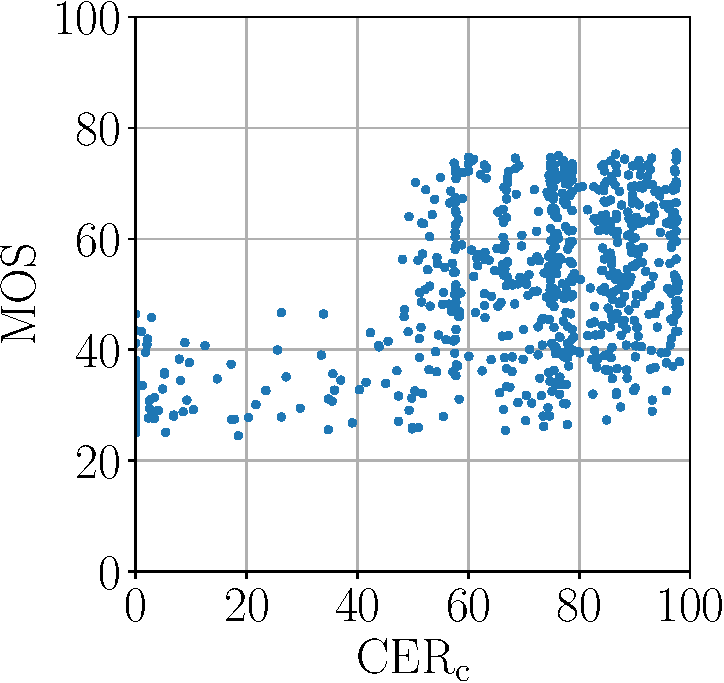
\includegraphics[width=\textwidth]{../../images/cer_mos_overview_gt_tess.pdf}
        \caption{CER vs MOS for Tesseract \gls{ocr} and the true \gls{gt}.}
        \label{fig:cer_vs_mos_gt_tess}
    \end{subfigure}
    \hfill
    \begin{subfigure}[b]{0.45\textwidth}
        \centering
        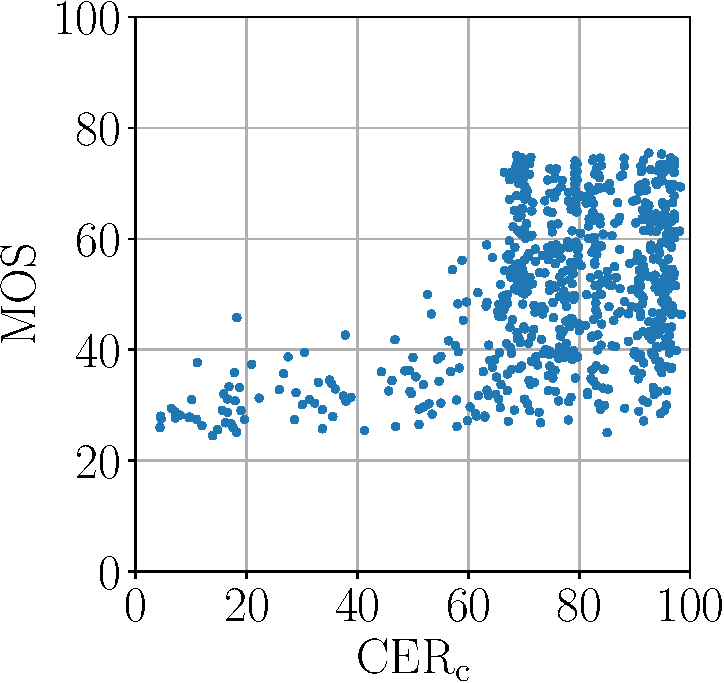
\includegraphics[width=\textwidth]{../../images/cer_mos_overview_gt_ezocr.pdf}
        \caption{CER vs MOS for EasyOCR and the true \gls{gt}.}
        \label{fig:cer_vs_mos_gt_ocr}
    \end{subfigure}
    \newline
    \begin{subfigure}[b]{0.45\textwidth}
        \centering
        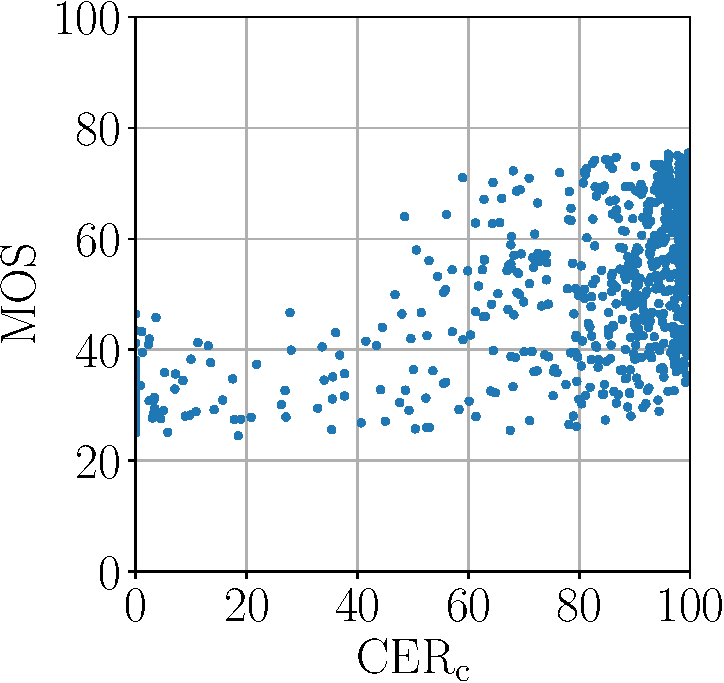
\includegraphics[width=\textwidth]{../../images/cer_mos_overview_ref_tess.pdf}
        \caption{CER vs MOS for Tesseract \gls{ocr} and the pseudo \gls{gt}.}
        \label{fig:cer_vs_mos_ref_tess}
    \end{subfigure}
    \hfill
    \begin{subfigure}[b]{0.45\textwidth}
        \centering
        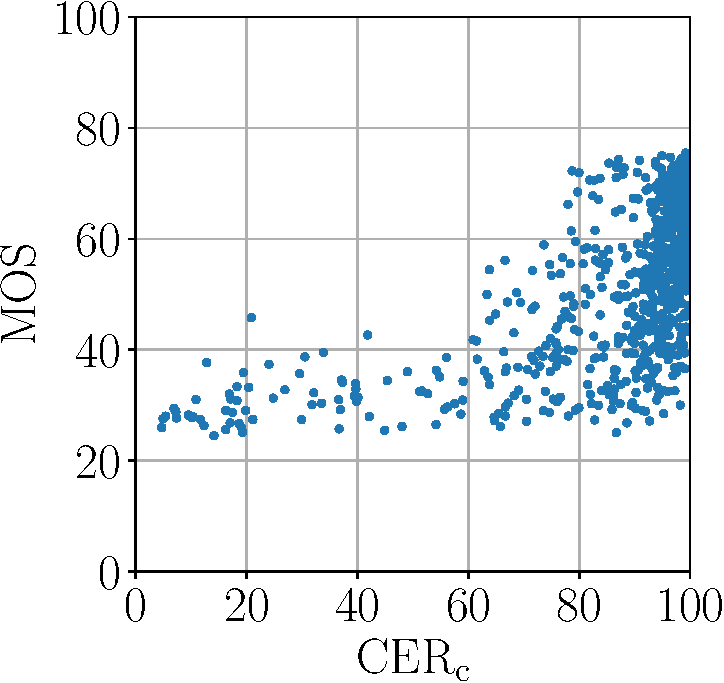
\includegraphics[width=\textwidth]{../../images/cer_mos_overview_ref_ezocr.pdf}
        \caption{CER vs MOS for EasyOCR and the pseudo \gls{gt}.}
        \label{fig:cer_vs_mos_ref_ocr}
    \end{subfigure}
    \caption{$\text{CER}_{\text{c}}$ vs \gls{mos} for Tesseract \gls{ocr} and EasyOCR, with the true \gls{gt} and the pseudo \gls{gt}.}
    \label{fig:cer_vs_mos_overview}
\end{figure}

In \autoref{fig:cer_vs_mos_overview} the $\text{CER}_{\text{c}}$ is plotted against the \gls{mos} for both \gls{ocr} algorithms and both \glspl{gt}.
Generally, we observe that the \gls{mos} ranges from 20 to 80 for all images.
On the other hand, the $\text{CER}_{\text{c}}$ spans from 0 to 100 for all images.
Comparing Tesseract \gls{ocr} with EasyOCR for the true \gls{gt}, we observe that the $\text{CER}_{\text{c}}$ distribution for Tesseract \gls{ocr} is more spread out with more lower $\text{CER}_{\text{c}}$ values compared to EasyOCR
Additionally, there are some points with zero $\text{CER}_{\text{c}}$ for Tesseract \gls{ocr}.
This implies that EasyOCR performs better in general and that Tesseract \gls{ocr} struggles with some distortions and fails to predict anything.
We notice similar behavior when comparing the pseudo \glspl{gt} for both \gls{ocr} algorithms, although the $\text{CER}_{\text{c}}$ values are generally higher.
This can be attributed to the fact that the predictions contains no additional errors due to positioning of the text elements and are generally closer to the pseudo \gls{gt} compared to the true \gls{gt}.


\section{Extension of the Dataset with Images Distorted by Compression Methods}
\label{sec:dataset_codec}

In this section, we first describe the extension of the dataset by encoding the reference image with the \gls{hevc} and \gls{vvc} codecs.

\subsection{High Efficiency Video Coding}
\label{subsec:hevc}

The \gls{hevc} \cite{hevc_2012} is one of the newest video codecs.
It is the successor of the H.264/MPEG-4 AVC codec.
The main improvements were the leveraging of parallel processing architecture in modern devices and addressing higher resolutions.
The codec uses the conventional approach of dividing the image into blocks for encoding and leveraging sequential frames to only encode the difference instead of the whole frame.
However it also employs a number of new techniques to provide around 50\% bit rate savings for equivalent quality.

\subsection{Versatile Video Coding}
\label{subsec:vvc}

The \gls{vvc} \cite{vvc_2021} is the successor of the \gls{hevc} and the most recent video codec.
It has another 50\% bit rate savings compared to the \gls{hevc} for equivalent quality.
Additionally, the versatility of the codec enables it to be used for a wider range of applications, including $360^{\circ}$ immersive video, high dynamic range, adaptive streaming with resolution changes and many more.


It is to note, that we use these codecs on images instead of videos, which means that we are not leveraging the full potential of the videos codecs.
Furthermore, we encoded the images with the default and the \gls{scc} configuration of the codecs to observe the difference.
The most important difference to the other distorted images is that there are no subjective scores available for these images.
However, we can use more images for the comparison of the codecs, as we do not need to select based on too much focus on graphical objects over the text elements.
For the experiments related to the codecs we select the images with,
\begin{equation}
    i \in {1, 2, 3, 4, 5, 6, 7, 8, 9, 11, 12, 13, 15, 16, 18, 19, 20, 21, 22, 23, 24, 25, 27, 29}.
\end{equation}
For both codecs, we encode these images with \glspl{qp} $\in {35, 40, 45, 50}$.
% --- deviating from VVC common test conditions, due to lack of changes in the CER for lower QP values
We subsequently employ the \gls{ocr} algorithms to predict text in these images, enabling us to compute the $\text{CER}_{\text{c}}$.
Afterwards, we visualize rate-distortion curves and calculate the \gls{bdrate}, as described in \autoref{subsec:bdrate}.
To summarize, the original dataset has a \gls{mos} for each image with various distortions.
We are expanding the dataset by encoding the images with the \gls{hevc} and \gls{vvc} codecs.
Now that we have all the parts to describe the experiments, we evaluate and discuss the results in the next chapter.
